\documentclass{article}[11pt]

\usepackage{amsmath}
\usepackage{amssymb}
\usepackage{nicefrac}

\usepackage{pdflscape}

\usepackage{upgreek}

\usepackage{bashful}

% No intendation
\setlength\parindent{0pt}

\usepackage{hyperref}

\usepackage{siunitx}
\sisetup{
  per-mode=fraction,
  fraction-function=\tfrac
}

\usepackage{listings}
  \lstset{
    basicstyle=\ttfamily,
    escapeinside=||,
    xleftmargin=1cm
  }

\usepackage{float}

\usepackage{longtable}

\usepackage{multirow}

\usepackage{tikz}
  \usetikzlibrary{patterns}
  \usetikzlibrary{arrows.meta}
  \usetikzlibrary{shapes.misc}
  \usetikzlibrary{calc}

\usepackage{pgfplots}

\usepackage{cleveref}
\crefmultiformat{equation}{(#2#1#3)}{ and~(#2#1#3)}{, (#2#1#3)}{ and~(#2#1#3)}


\usepackage{acronym}
\usepackage[acronym,nonumberlist]{glossaries}
\glsdisablehyper
\makeglossaries
\newacronym{spice}{SPICE}{Simulation Program with Integrated Circuit Emphasis}
\newacronym{lef}{LEF}{Library Exchange Format}
\newacronym{dft}{DFT}{Discrete Fourier Transform}
\newacronym{dtft}{DTFT}{Discrete-Time Fourier Transform}
\newacronym{fft}{FFT}{Fast Fourier Transform}
\newacronym{mosfet}{MOSFET}{Metal–Oxide–Semiconductor Field-Effect Transistor}
\newacronym{clm}{CLM}{Channel Length Modulation}
\newacronym{de}{DE}{differential equation}
\newacronym{soi}{SOI}{silicon-on-insulator}
\newacronym{ldo}{LDO}{low-dropout regulator}
\newacronym{ota}{OTA}{operational-transconductance amplifier}
\newacronym{ofa}{OFA}{operational-floating amplifier}

% literature
\usepackage[ backend=biber
           , isbn=true
           , sorting=none
           , style=ieee
           ]{biblatex}
\addbibresource{./../../literature.bib}

% definitions
\def \whatis       {Notes}
\def \title        {Fuubar}

\def \author       {Matthias Schweikardt}

\def \authorMail   {mschweikardt@posteo.de}

\def \authorGithub {mschweikardt}

\def \license      {CC BY-SA 4.0}
\def \licenseUrl   {https://creativecommons.org/licenses/by-sa/4.0/}

\def \date         {nodate}

\def \pdfurl       {https://mschweikardt.github.io/ee-notes/%
\bash[stdout]
IFS=/ 
var=($PWD)
echo ${var[-1]}
\END%
.pdf
}
\def \srcurl       {srcurl}


% Customize footer and header of document
\usepackage{fancyhdr}

% Access last page number
\usepackage{lastpage}

% Access last page number
\usepackage[thinc]{esdiff}

% Physics
\usepackage{physics}

% Comment environment
\usepackage{comment}

% Subcaptions
\usepackage{subcaption}

% Thicker lines in tables
\usepackage{booktabs}

% Indentation in footnote
\makeatletter
\renewcommand\@makefntext[1]{\leftskip=2em\hskip-0.5em\@makefnmark#1}
\makeatother         

% qty with the siunitx definition
\AtBeginDocument{\RenewCommandCopy\qty\SI}

% TikZ compatibility
\pgfplotsset{compat=1.18}


\makeatletter
\pgfmathdeclarefunction{myatan2}{2}{%
\begingroup%
  \pgfmathfloattofixed{#1}\edef\tempa{\pgfmathresult}%
  \pgfmathfloattofixed{#2}%
  \pgfkeys{pgf/fpu=false}%
  \pgfmathparse{atan2(\tempa,\pgfmathresult)}\pgfkeys{/pgf/fpu}%
  \pgfmathfloatparsenumber{\pgfmathresult}%
  \pgfmath@smuggleone\pgfmathresult%
\endgroup
}
\makeatother

\usepackage{tabularx}
% usepackages
\usepackage[ a4paper
           , textwidth  = 16.0cm
           , textheight = 25.0cm
           , headsep    =  0.25cm
           , voffset    =  0.3cm
           , footskip   =  1.25cm
           ]{geometry}

% Section and subsection enumeration
\renewcommand{\thesection}{\Roman{section}.} 
\renewcommand{\thesubsection}{\thesection\Alph{subsection}}

\usepackage{titlesec}
\titleformat{\section}
  {\normalfont\Large\bfseries}{\thesection}{0.2em}{}
\titleformat{\subsection}
  {\normalfont\large\bfseries}{\thesubsection}{0.2em}{}


% Defince title of document
\newcommand{\notetitle}{
  \begingroup
  \hypersetup{hidelinks}
  \thispagestyle{notefirst}
  \begin{center}
  \rule{\textwidth}{1pt}\\
  \medskip
  {\it \whatis}\\
  \bigskip
  {\LARGE \textbf{\title}}\\
  \medskip
  {\small \author}\\
  \rule{\textwidth}{0.5pt}\\
  {\small
    \begin{minipage}[t]{0.5\textwidth}
      \begin{tabular}[t]{ p{2.25cm} p{5.75cm}}
        Mail: & \href{mailto:\authorMail}{\tt{\authorMail}} \\
        Github: & \href{https://github.com/\authorGithub}{\tt{\authorGithub}} \\
      \end{tabular}
    \end{minipage}%
    %
    \begin{minipage}[t]{0.5\textwidth}
      \begin{tabular}[t]{ p{2.25cm} p{5.75cm} }
        Date: & \date  \\
        License: & \href{\licenseUrl}{\license}
      \end{tabular}
    \end{minipage}
  }%
  {\small
    \begin{minipage}[t]{\textwidth}
      \begin{tabular}[t]{ p{2.25cm} p{12cm}}
        Latest PDF: & \href{\pdfurl}{\tt{\pdfurl}} \\
        Latest Source: & \href{\srcurl}{\tt{\srcurl}}
      \end{tabular}
    \end{minipage}%
  }
  \bigskip
  \rule{\textwidth}{1pt}
  \end{center}
  \endgroup
}

% Header and footer on first page
\fancypagestyle{notefirst}{
  \fancyhf{}
  \renewcommand{\headrulewidth}{0pt}
  \renewcommand{\footrulewidth}{0pt}

  \fancyfoot[C]{\thepage/\pageref*{LastPage}}
}

% Header and footer on 2nd-last page
\fancypagestyle{noterest}{
  \fancyhf{}
  \renewcommand{\headrulewidth}{0.5pt}
  \renewcommand{\footrulewidth}{0.0pt}

  \fancyhead[L]{\author}
  \fancyhead[C]{\title}
  \fancyhead[R]{\date}

  \fancyfoot[C]{\thepage/\pageref*{LastPage}}
}
\pagestyle{noterest}

\usepackage{amsmath}
\usepackage{amssymb}
\usepackage{nicefrac}

\usepackage{pdflscape}

\usepackage{upgreek}

\usepackage{bashful}

% No intendation
\setlength\parindent{0pt}

\usepackage{hyperref}

\usepackage{siunitx}
\sisetup{
  per-mode=fraction,
  fraction-function=\tfrac
}

\usepackage{listings}
  \lstset{
    basicstyle=\ttfamily,
    escapeinside=||,
    xleftmargin=1cm
  }

\usepackage{float}

\usepackage{longtable}

\usepackage{multirow}

\usepackage{tikz}
  \usetikzlibrary{patterns}
  \usetikzlibrary{arrows.meta}
  \usetikzlibrary{shapes.misc}
  \usetikzlibrary{calc}

\usepackage{pgfplots}

\usepackage{cleveref}
\crefmultiformat{equation}{(#2#1#3)}{ and~(#2#1#3)}{, (#2#1#3)}{ and~(#2#1#3)}


\usepackage{acronym}
\usepackage[acronym,nonumberlist]{glossaries}
\glsdisablehyper
\makeglossaries
\newacronym{spice}{SPICE}{Simulation Program with Integrated Circuit Emphasis}
\newacronym{lef}{LEF}{Library Exchange Format}
\newacronym{dft}{DFT}{Discrete Fourier Transform}
\newacronym{dtft}{DTFT}{Discrete-Time Fourier Transform}
\newacronym{fft}{FFT}{Fast Fourier Transform}
\newacronym{mosfet}{MOSFET}{Metal–Oxide–Semiconductor Field-Effect Transistor}
\newacronym{clm}{CLM}{Channel Length Modulation}
\newacronym{de}{DE}{differential equation}
\newacronym{soi}{SOI}{silicon-on-insulator}
\newacronym{ldo}{LDO}{low-dropout regulator}
\newacronym{ota}{OTA}{operational-transconductance amplifier}
\newacronym{ofa}{OFA}{operational-floating amplifier}

% literature
\usepackage[ backend=biber
           , isbn=true
           , sorting=none
           , style=ieee
           ]{biblatex}
\addbibresource{./../../literature.bib}

% definitions
\def \whatis       {Notes}
\def \title        {Fuubar}

\def \author       {Matthias Schweikardt}

\def \authorMail   {mschweikardt@posteo.de}

\def \authorGithub {mschweikardt}

\def \license      {CC BY-SA 4.0}
\def \licenseUrl   {https://creativecommons.org/licenses/by-sa/4.0/}

\def \date         {nodate}

\def \pdfurl       {https://mschweikardt.github.io/ee-notes/%
\bash[stdout]
IFS=/ 
var=($PWD)
echo ${var[-1]}
\END%
.pdf
}
\def \srcurl       {srcurl}


% Customize footer and header of document
\usepackage{fancyhdr}

% Access last page number
\usepackage{lastpage}

% Access last page number
\usepackage[thinc]{esdiff}

% Physics
\usepackage{physics}

% Comment environment
\usepackage{comment}

% Subcaptions
\usepackage{subcaption}

% Thicker lines in tables
\usepackage{booktabs}

% Indentation in footnote
\makeatletter
\renewcommand\@makefntext[1]{\leftskip=2em\hskip-0.5em\@makefnmark#1}
\makeatother         

% qty with the siunitx definition
\AtBeginDocument{\RenewCommandCopy\qty\SI}

% TikZ compatibility
\pgfplotsset{compat=1.18}


\makeatletter
\pgfmathdeclarefunction{myatan2}{2}{%
\begingroup%
  \pgfmathfloattofixed{#1}\edef\tempa{\pgfmathresult}%
  \pgfmathfloattofixed{#2}%
  \pgfkeys{pgf/fpu=false}%
  \pgfmathparse{atan2(\tempa,\pgfmathresult)}\pgfkeys{/pgf/fpu}%
  \pgfmathfloatparsenumber{\pgfmathresult}%
  \pgfmath@smuggleone\pgfmathresult%
\endgroup
}
\makeatother

\usepackage{tabularx}

\def \title  {EKV MOSFET Model}
\def \date   {July 28, 2025}

\def \pdfurl {https://mschweikardt.github.io/ee-notes/ekv.pdf}
\def \srcurl {https://github.com/mschweikardt/ee-notes/tree/main/notes/ekv}

\usepackage[scale=5]{draftwatermark}

\begin{document}

\notetitle

EKV%
\footnote{Named by their inventors Enz, Krummenacher and Vittoz}
is an analytical \gls{mosfet} model \cite{enz-ekv-95,enz-ekvstory-08}.
The drain current of the transistor is given by
\begin{equation}
I_{\mathrm{D}} = I_{\mathrm{S}} \left(\mathrm{IC}_{\mathrm{F}}-\mathrm{IC}_{\mathrm{R}}\right),
\end{equation}
with the specific current $I_{\mathrm{S}}$ (unit A), the forward 
inversion coefficient 
$\mathrm{IC}_{\mathrm{F}}(V_{\mathrm{G}}, V_{\mathrm{S}})$ (unitless) and 
the backward inversion coefficient 
$\mathrm{IC}_{\mathrm{R}}(V_{\mathrm{G}}, V_{\mathrm{D}})$ (unitless).
The inversion coefficient $\mathrm{IC}$ is a proxy for the inversion level of 
the channel of the \gls{mosfet}.

\medskip

The specific current is given by
\begin{equation}
  I_{\mathrm{S}} = 2 n V_{\mathrm{T}}^2 K' \frac{W}{L},
\end{equation}
with the temperature voltage $V_{\mathrm{T}}$%
\footnote{$V_{\mathrm{T}}=\frac{k_{\mathrm{B}} T }{e}$, with the 
Boltzmann constant $k_{\mathrm{B}}=\SI{1.38d-23}{\joule\per\kelvin}$, 
the absolute temperature $T$ in \si{\kelvin} and the 
elementary charge $e=\SI{1.6025d-19}{\ampere\second}$.},
the subthreshold slope $n$%
\footnote{$n$ is between 1.2 and 1.5 in a bulk technology and smaller 
for \gls{soi} transistors\cite{jespers-gmid-17}.}
 and the transconductance coefficient $K'$ 
(conf. \cite{mosfet-square-law}).
Here, we will only investigate the forward region, so 
$\mathrm{IC}_{\mathrm{R}} \rightarrow 0$.

\bigskip

The forward inversion coefficient is given by 
(subscript $\mathrm{F}$ omitted)

\begin{equation}\label{eq:ic}
  \mathrm{IC} = \ln\left(1+\exp\left\{\frac{V_{\mathrm{G}}-V_{\mathrm{S}}-V_{\mathrm{TH}}}{2 n V_{\mathrm{T}}}\right\}\right)^2
              = \ln\left(1+\exp\left\{\frac{V_{\mathrm{GS}}-V_{\mathrm{TH}}}{2 n V_{\mathrm{T}}}\right\}\right)^2.
\end{equation}


When $V_{\mathrm{GS}}-V_{\mathrm{TH}} \gg 0$, we can approximate 
it with

\begin{equation}\label{eq:ic-quad}
  \mathrm{IC}_{\mathrm{quad}} = \left(\frac{V_{\mathrm{GS}}-V_{\mathrm{TH}}}{2 n V_{\mathrm{T}}}\right)^2
\end{equation}

and for $V_{\mathrm{GS}}-V_{\mathrm{TH}} \ll 0$ with

\begin{equation}\label{eq:ic-exp}
  \mathrm{IC}_{\mathrm{exp}} = \exp\left\{\frac{V_{\mathrm{GS}}-V_{\mathrm{TH}}}{n V_{\mathrm{T}}}\right\}.
\end{equation}

$\mathrm{IC}_{\mathrm{quad}}$ is quadratic and is therefore a 
reasonable approximation for the \textit{saturation} region, while 
$\mathrm{IC}_{\mathrm{exp}}$ is exponential and is a good 
approximation for the \textit{subthreshold} region.
Fig. \ref{fig:plot} plots \eqref{eq:ic}, \eqref{eq:ic-quad} and  
\eqref{eq:ic-exp}.

\begin{figure}[ht]
  \centering
  \begin{tikzpicture}
    \input{./../../tikzlib/figs/ekv-ic-vs-vgseff.tex}
  \end{tikzpicture}
  \caption{$\mathrm{IC}$, $\mathrm{IC}_{\mathrm{exp}}$ and 
    $\mathrm{IC}_{\mathrm{quad}}$ as a function of 
    $\frac{V_{\mathrm{GS}}-V_{\mathrm{TH}}}{n V_{\mathrm{T}}}$ with added 
    inversion regions}
  \label{fig:plot}
\end{figure}

Neither $\mathrm{IC}_{\mathrm{quad}}$ or $\mathrm{IC}_{\mathrm{exp}}$
are sufficient to approximate the behavior of the $\mathrm{IC}$
close to $V_{\mathrm{GS}}=V_{\mathrm{TH}}$.

\bigskip

Tab.~\ref{tab:ekv-regions} summarizes the individual $\mathrm{IC}$ ranges,
their corresponding inversion level and curvature.
\begin{table}[h]
\centering
\caption{EKV regions}
\begin{tabular}{ccccc}
\toprule
Identifier & Name               & $\mathrm{IC}$  & Curvature    & Current             \\ \midrule
S.I.       & strong inversion   & $\geq 10$      & quadratic    & drift               \\ 
M.I.       & moderate inversion & $0.1$-$10$     & -            & drift and diffusion \\ 
W.I.       & weak inversion     & $\leq 0.1$     & exponential  & diffusion           \\ \toprule
\end{tabular}
\label{tab:ekv-regions}
\end{table}

\bigskip

The drain current in \textit{strong inversion} is
\begin{equation}\label{eq:id-si}
  I_{\mathrm{D,S.I.}} = I_{\mathrm{S}} \cdot \mathrm{IC}_{\mathrm{quad}}
                      = 2 n V_{\mathrm{T}}^2 K' \frac{W}{L} \cdot \left(\frac{V_{\mathrm{GS}}-V_{\mathrm{TH}}}{2 n V_{\mathrm{T}}}\right)^2
                        \stackrel{n=1}{=} \frac{1}{2} K' \frac{W}{L} \left(V_{\mathrm{GS}}-V_{\mathrm{TH}}\right)^2
\end{equation}
and matches the square law in the saturation region 
\cite{mosfet-square-law}.

\bigskip

The transconductance is
\begin{equation}\label{eq:gm}
\begin{split}
 g_{\mathrm{m}}
 &= \frac{\mathrm{d} I_{\mathrm{D}}}{\mathrm{d} V_{\mathrm{GS}}} \\
 &= \frac{I_{\mathrm{S}}}{n V_{\mathrm{T}}} \frac{\exp\left\{\frac{V_{\mathrm{GS}}-V_{\mathrm{TH}}}{2 n V_{\mathrm{T}}}\right\}}{\exp\left\{\frac{V_{\mathrm{GS}}-V_{\mathrm{TH}}}{2 n V_{\mathrm{T}}}\right\}+1} \ln\left(1+\exp\left\{\frac{V_{\mathrm{GS}}-V_{\mathrm{TH}}}{2 n V_{\mathrm{T}}}\right\}\right)\\
 &= \frac{I_{\mathrm{S}}}{n V_{\mathrm{T}}} \left(1-\exp\left\{-\sqrt{\mathrm{IC}}\right\}\right) \sqrt{\mathrm{IC}}
\end{split}
\end{equation}
and therefore the efficiency
\begin{equation}\label{eq:gmid}
\frac{g_{\mathrm{m}}}{I_{\mathrm{D}}} = \frac{1}{n V_{\mathrm{T}}}  \frac{1-\exp\left\{-\sqrt{\mathrm{IC}}\right\}}{\sqrt{\mathrm{IC}}}.
\end{equation}
A plot of the normalized efficiency $\frac{g_{\mathrm{m}}}{I_{\mathrm{D}}} n V_{\mathrm{T}}$
is provided in Fig.~\ref{fig:plot2}.
\begin{figure}[ht]
  \centering
  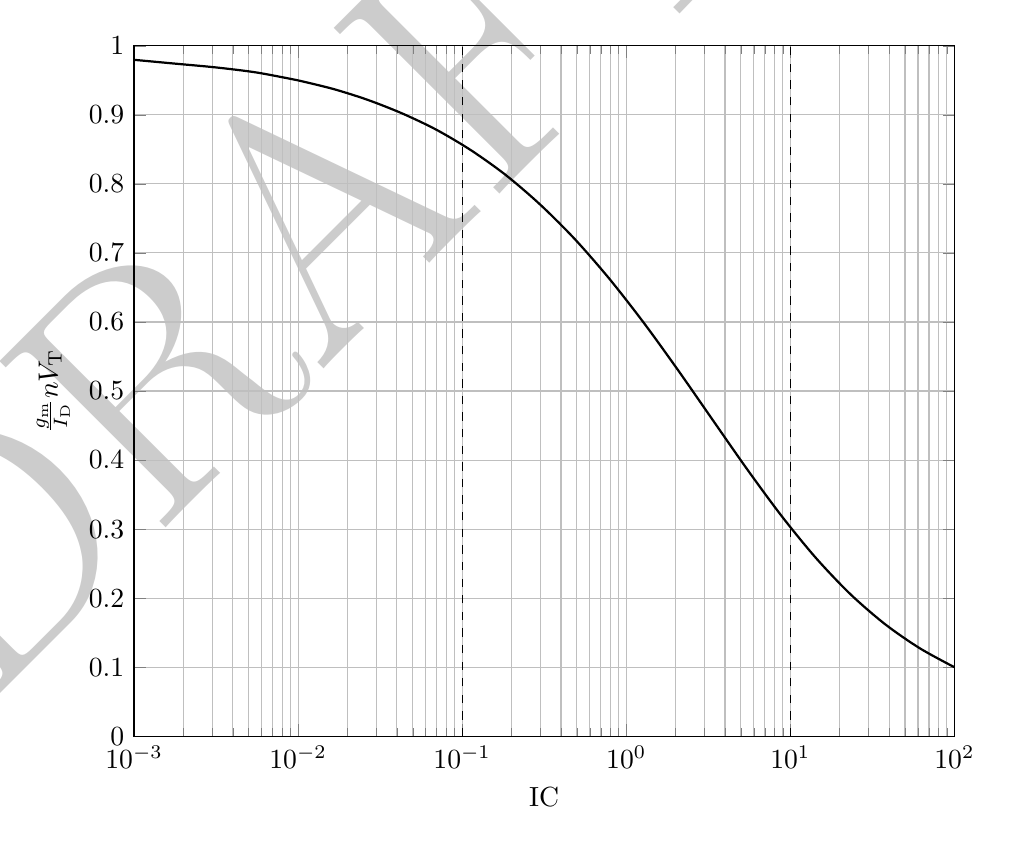
\begin{tikzpicture}
    \begin{axis}[ ylabel=$\frac{g_{\mathrm{m}}}{I_{\mathrm{D}}} n V_{\mathrm{T}}$
                , xlabel=$\mathrm{IC}$
                , xmode=log
                , ymin=0
                , ymax=1
                , xmin=0.001
                , xmax=100
                , clip=true
                , grid=both
                , width= 12cm
                ]

    \draw[dashed] (axis cs:0.1,0) -- (axis cs:0.1,1);
    \draw[dashed] (axis cs:10,0) -- (axis cs:10,1);

   \addplot[ mark=none
           , thick
           , domain=0.001:0.01
           , samples=5
           , smooth
           , thick] {(1-exp(-sqrt(x)))/sqrt(x)}; 
    \addplot[ mark=none
            , thick
            , domain=0.01:100
            , samples=20
            , smooth
            , thick] {(1-exp(-sqrt(x)))/sqrt(x)}; 
    \end{axis}
  \end{tikzpicture}
  \caption{Normalized efficiency 
    $\frac{g_{\mathrm{m}}}{I_{\mathrm{D}}} n V_{\mathrm{T}}$ vs. 
    inversion coefficient $\mathrm{IC}$}
  \label{fig:plot2}
\end{figure}
A series expansion of \eqref{eq:gmid} is
\begin{equation}\label{eq:gmid-exp}
\frac{g_{\mathrm{m}}}{I_{\mathrm{D}}} \approx \frac{1}{n V_{\mathrm{T}}} \left(1- \frac{\sqrt\mathrm{IC}}{2} + \frac{\mathrm{IC}}{6} - \frac{\mathrm{IC}^{\nicefrac{3}{2}}}{24} + \mathcal{O}(\mathrm{IC}^2)\right).
\end{equation}
It converges to $\nicefrac{1}{n V_{\mathrm{T}}}$ when $\mathrm{IC} \rightarrow 0$.
Therefore, the maximum efficiency a transistor can achieve is
\begin{equation}\label{eq:gmid-max}
\frac{g_{\mathrm{m}}}{I_{\mathrm{D}}}\bigg|_{\mathrm{max}} = \frac{1}{n V_{\mathrm{T}}},
\end{equation}
which is about \SI{25.8}{\per\volt}-\SI{38.7}{\per\volt} at 
room temperature (\SI{300}{\kelvin}).

\printbibliography

\end{document}